A complete example of how to run the \glsentryfull{qmla} framework, 
    including how to implement a custom \glsentryfull{es}, 
    and generate/interpret analysis, is given.
\par 

First, \emph{fork} the \gls{qmla} codebase from \cite{flynn2021QMLA}\footnotemark.
\footnotetext{This will require a Github account.} 
Now, we must download the code base and ensure it runs properly;
    these instructions are implemented via the command line\footnotemark. 
\footnotetext{
    Note: these instructions are tested for Linux and presumed to work on Mac, but untested on Windows. 
    It is likely some of the underlying software (redis servers) can not be installed on Windows. 
}
    
\begin{lstlisting}[
    label=listing:qmla_setup,
    caption={QMLA codebase setup},
    language=Bash
]
# Install redis (database broker)
sudo apt update
sudo apt install redis-server
 
# make directory for QMLA
cd
mkdir qmla_test
cd qmla_test

# make Python virtual environment for QMLA
# note: change Python3.6 to desired version
sudo apt-get install python3.6-venv 
python3.6 -m venv qmla-env    
source qmla-env/bin/activate

# Download QMLA
git clone --depth 1 https://github.com/username/QMLA.git # REPLACE username

# Install dependencies
cd QMLA 
pip install -r requirements.txt 
\end{lstlisting}

Note there may be a problem with some packages in the \ttt{requirements.txt} arising from the attempt to install them all through
a single call to \ttt{pip install}. 
Ensure these are all installed before proceeding. 
\par 

When all of the requirements are installed, test the framework runs. 
\gls{qmla} uses \ttt{redis} databases to store intermittent data:
    we must manually initialise the database. 
Run the following 
    (note: here we list \ttt{redis-4.0.8}, but this must be corrected to reflect the 
    version installed on the user's machine in the above setup section):
\begin{lstlisting}[
    label=listing:athlete_class,
    caption={Launch redis database},
    language=Bash
]
~/redis-4.0.8/src/redis-server
\end{lstlisting}

which should give something like \cref{fig:terminal_redis}.
\begin{figure}[h!]
    \begin{center}
        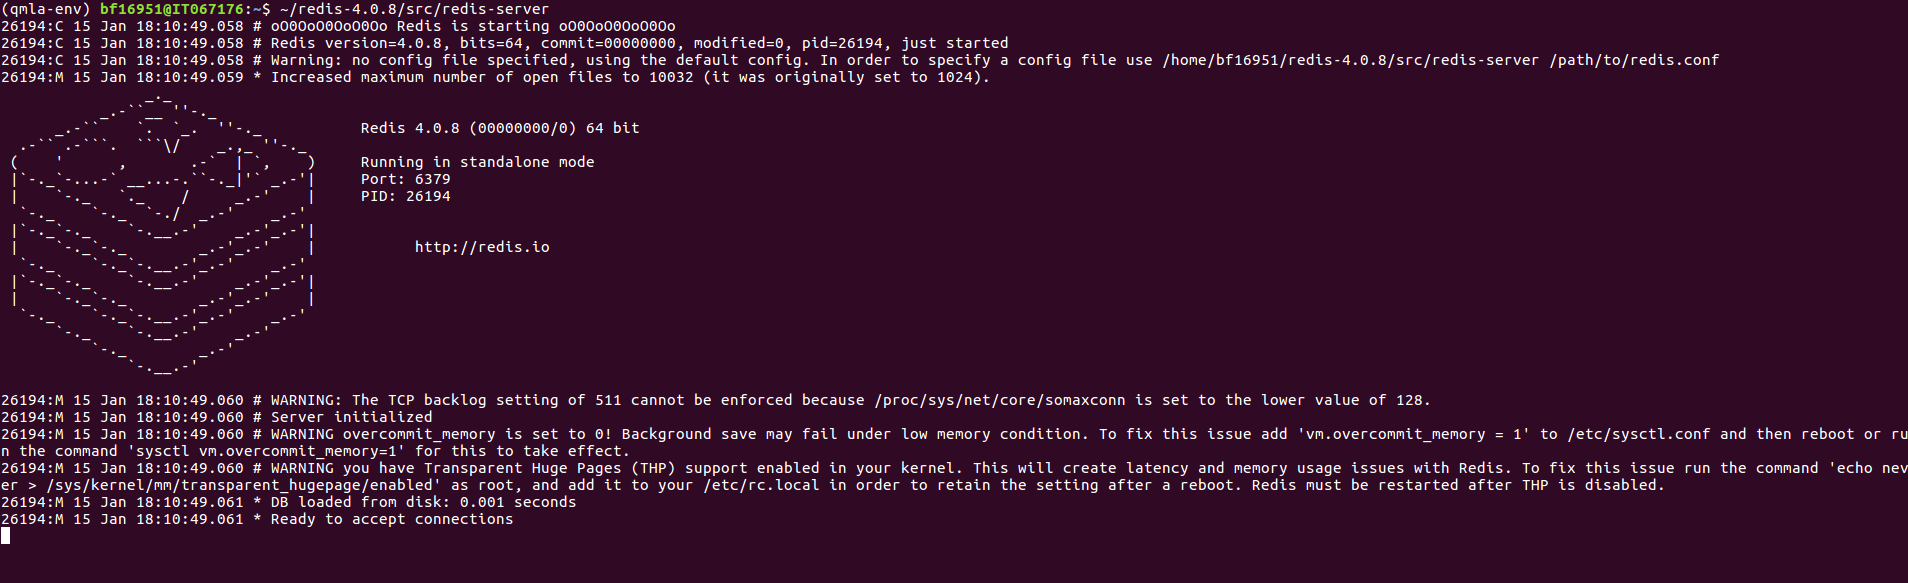
\includegraphics[width=0.9\textwidth]{appendix/figures/terminal_redis.png}
    \end{center}
    \caption[Terminal running redis-server]{Terminal running \ttt{redis-server}.}
    \label{fig:terminal_redis}
\end{figure}
\par 

In a text editor, open \ttt{qmla\_test/QMLA/launch/local\_launch.sh}; 
    here we will ensure that we are running the \gls{qhl} algorithm, 
    with 5 experiments and 20 particles, on the \gls{es} named \ttt{ExampleBasic}.
Ensure the first few lines of \ttt{local\_launch.sh} read:

\begin{lstlisting}[
    label=listing:local_launch,
    caption={\ttt{local\_launch} script},
    language=Bash
]
    
#!/bin/bash

###############
# QMLA run configuration
###############
num_instances=1
run_qhl=1 # perform QHL on known (true) model
run_qhl_multi_model=0 # perform QHL for defined list of models.
exp=5 # number of experiments
prt=20 # number of particles

###############
# QMLA settings - user
###############
plot_level=5
debug_mode=0

###############
# QMLA settings - default
###############
do_further_qhl=0 # QHL refinement to best performing models 
q_id=0 # isntance ID can start from other ID if desired
use_rq=0
further_qhl_factor=1
further_qhl_num_runs=$num_instances
plots=0
number_best_models_further_qhl=5

###############
# Choose an exploration strategy 
# This will determine how QMLA proceeds. 
###############

exploration_strategy="ExampleBasic"
\end{lstlisting}    

Now we can run 
Ensure the terminal running redis is kept active, and open a separate terminal window. 
We must activate the Python virtual environment configured for \gls{qmla}, 
which we set up in \cref{listing:qmla_setup}. 
Then, we navigate to the \gls{qmla} directory, and launch:
\begin{lstlisting}[
    label=listing:launch_example,
    caption={Launch QMLA},
    language=Bash
]

# activate the QMLA Python virtual environment 
source qmla_test/qmla-env/bin/activate

# move to the QMLA directory 
cd qmla_test/QMLA
# Run QMLA
cd launch   
./local_launch.sh

\end{lstlisting}

There may be numerous warnings, but they should not affect whether \gls{qmla} has succeeded; 
    \gls{qmla} will \ttt{raise} any significant error. 
Assuming the run has completed successfully, \gls{qmla} stores the run's results in a subdirectory
    named by the date and time it was started.  
For example, if the run was initialised on January $1^{st}$ at 01:23, navigate to the corresponding directory by

\begin{lstlisting}[
    label=listing:results_directory,
    caption={QMLA results directory},
    language=Bash
]
cd results/Jan_01/01_23
\end{lstlisting}

For now it is sufficient to notice that the code has sun successfully and the analysis has generated several new files and directores; 
    in the following sections we will describe the outputs. 

\section{Custom \glsentrylong{es}}

Next, we design a basic \gls{es}, for the purpose of demonstrating how to run the algorithm.
\glspl{es} are placed in the directory \ttt{qmla/exploration\_strategies}. 
To make a new one, navigate to the exploration strategies directory, 
make a new subdirectory, and copy the template file. 

\begin{lstlisting}[
    label=listing:athlete_class,
    caption={QMLA codebase setup},
    language=Bash
]

cd ~/qmla_test/QMLA/exploration_strategies/
mkdir custom_es

# Copy template file into example
cp template.py custom_es/example.py
cd custom_es

\end{lstlisting}

Ensure \gls{qmla} will know where to find the \gls{es} by importing everything from the custom \gls{es} 
    directory into to the main \ttt{exploration\_strategy} module. 
Then, in the \ttt{custom\_es} directory, make a file called \ttt{\_\_init\_\_.py} which imports the new \gls{es}
    from the \ttt{example.py} file. 
To add any further \glspl{es} inside the directory \ttt{custom\_es}, include them in the custom \ttt{\_\_init\_\_.py},
    and they will automatically be available to \gls{qmla}.

\begin{lstlisting}[
    label=listing:importing_es,
    caption={Providing custom exploration strategy to QMLA},
    language=Python
]

# inside qmla/exploration_strategies/custom_es
#  __init__.py    
from qmla.exploration_strategies.custom_es.example import *

# inside qmla/exploration_strategies, add to the existing
# __init__.py 
from qmla.exploration_strategies.custom_es import *

\end{lstlisting}

Now, change the structure (and name) of the \gls{es} inside \ttt{custom\_es/example.py}. 
Say we wish to target the true model 
\begin{equation}
    \label{eqn:example_es_true_ham}
    \begin{split}
        \al &= \irow{ \alpha_{1,2} & \alpha_{2,3} & \alpha_{3,4}} \\
        \terms &= \icol{ \sz^1 \otimes \sz^2 \\ \sz^2 \otimes \sz^3  \\ \sz^3 \otimes \sz^4 } \\
        \Longrightarrow \ho &= \sz^{(1,2)} \sz^{(2,3)} \sz^{(3,4)} \\
    \end{split}
\end{equation}

\gls{qmla} interprets models as strings, where terms are separated by \ttt{+}, and parameters are implicit. 
So the target model in \cref{eqn:example_es_true_ham} will be given by 
$$ \ttt{pauliSet\_1J2\_zJz\_d4+pauliSet\_2J3\_zJz\_d4+pauliSet\_3J4\_zJz\_d4}. $$

Adapting the template \gls{es} slightly, we can define a model generation strategy with a small number of hard coded 
    candidate models introduced at the first of the \glsentrylong{et}. 
We will also set the parameters of the terms which are present in $\ho$, as well as the range in which to search parameters.
Keeping the \ttt{import}s at the top of the \ttt{example.py}, rewrite the \gls{es} as: 

\begin{lstlisting}[
    label=listing:basic_es,
    caption={QMLA ExampleBasic explorattion strategy},
    language=Python
]
class ExampleBasic(
    exploration_strategy.ExplorationStrategy
):

    def __init__(
        self,
        exploration_rules,
        true_model=None,
        **kwargs
    ):
        self.true_model = 'pauliSet_1J2_zJz_d4+pauliSet_2J3_zJz_d4+pauliSet_3J4_zJz_d4'
        super().__init__(
            exploration_rules=exploration_rules,
            true_model=self.true_model,
            **kwargs
        )

        self.initial_models = None
        self.true_model_terms_params = {
            'pauliSet_1J2_zJz_d4' : 2.5,
            'pauliSet_2J3_zJz_d4' : 7.5,
            'pauliSet_3J4_zJz_d4' : 3.5,
        }
        self.tree_completed_initially = True
        self.min_param = 0
        self.max_param = 10

    def generate_models(self, **kwargs):

        self.log_print(["Generating models; spawn step {}".format(self.spawn_step)])
        if self.spawn_step == 0:
            # chains up to 4 sites
            new_models = [
                'pauliSet_1J2_zJz_d4',
                'pauliSet_1J2_zJz_d4+pauliSet_2J3_zJz_d4',
                'pauliSet_1J2_zJz_d4+pauliSet_2J3_zJz_d4+pauliSet_3J4_zJz_d4',
            ]
            self.spawn_stage.append('Complete')

        return new_models

\end{lstlisting}


To run\footnotemark \ the example \gls{es} for a meaningful tests, 
    return to the \ttt{local\_launch} of \cref{listing:local_launch}, 
    but change some of the settings:
\begin{lstlisting}[
    label=listing:example_es_qhl_run,
    caption={\ttt{local\_launch} configuration for QHL.},
    language=Bash
]
prt=2000
exp=500
run_qhl=1
exploration_strategy=ExampleBasic
\end{lstlisting}

Run locally again as in \cref{listing:launch_example};
    then move to the results directory as in \cref{listing:results_directory}. 
\footnotetext{
    Note this will take up to 15 minutes to run. 
    This can be reduced by lowering the values of \ttt{prt}, \ttt{exp}, 
    which is sufficient for testing but note that the outcomes will be less effective 
    than those presented in the figures of this section.
}
\par 
\gls{qmla} stores results, and generates plots, 
    over the entire range of the algorithm\footnotemark, i.e. the \gls{run}, \gls{instance} and models. 
\footnotetext{Recall that a single implementation of \gls{qmla} is called an \gls{instance},    
    while a series of instances which share the same target model is called the \gls{run}.}
The depth of analysis performed automatically is set by the user control \ttt{plot\_level} in \ttt{local\_launch.sh};
    for \ttt{plot\_level=1}, only the most crucial figures are generated, while \ttt{\plot\_level=6} generates plots for every individual 
    model considered. 
For model searches across large model spaces and/or considering many candidates,
    excessive plotting can cause considerable slow-down, so users should be careful to generate plots only 
    to the degree they will be useful. 
Next we show some examples of the available plots. 
\par 

\subsection{Model analysis}

We have just run \glsentryfull{qhl} for the model in \cref{eqn:example_es_true_ham} for a single instance, 
    using a reasonable number of particles and experiments, so we expect to have trained the model well. 
Instance-level results are stored (e.g. for the instance with \ttt{qmla\_id=1}) in \ttt{Jan\_01/01\_23/instances/qmla\_1}.
Individual models' insights can be found in \ttt{model\_training}, 
    e.g. the model's \ttt{learning\_summary} \cref{fig:qmla_learning_summary}, and \ttt{dynamics} in \cref{fig:qmla_model_dynamics}.
\par 

\begin{figure}[H]
    \begin{center}
    \subfloat[]{
        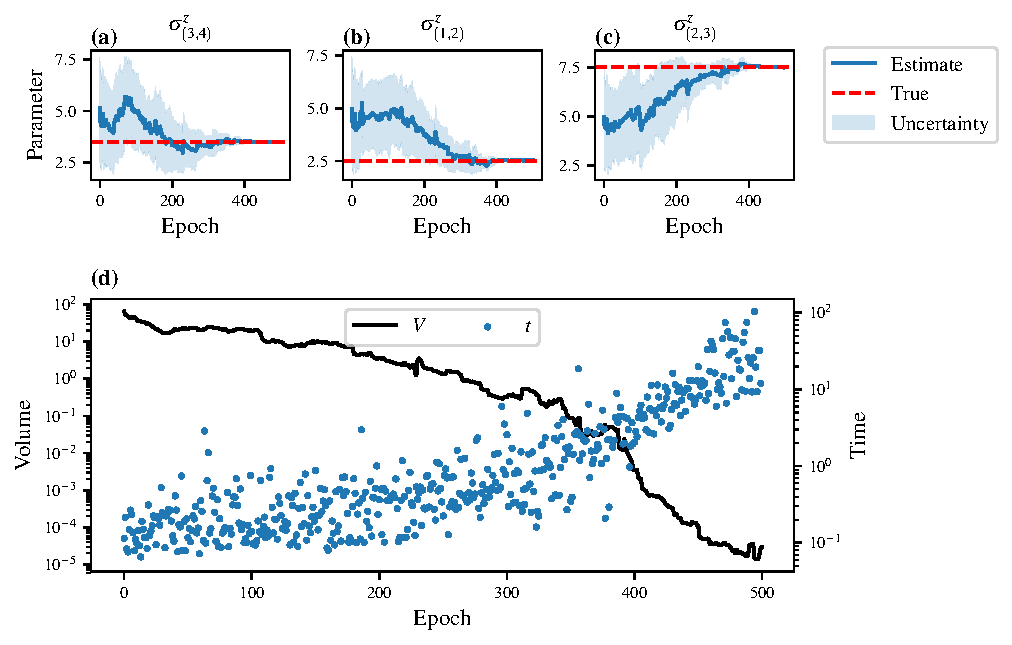
\includegraphics[width=0.75\textwidth]{qmla_run_data/Jan_17/18_04/instances/qmla_1/model_training/learning_summary_1.pdf}
        \label{fig:qmla_learning_summary}
    }
    \qquad
    \subfloat[]{
        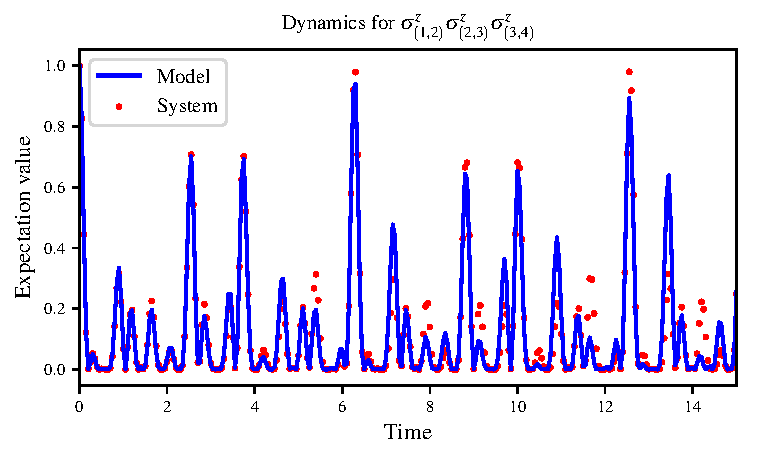
\includegraphics[width=0.75\textwidth]{qmla_run_data/Jan_17/18_04/instances/qmla_1/model_training/dynamics_1.pdf}
        \label{fig:qmla_model_dynamics}
    }
    \end{center}
    \caption[ Instance plots]{
        Instance plots, stored in (for example) \ttt{Jan\_01/01\_23/instances/qmla\_1/model\_training}. 
        \textbf{a} \ttt{learning\_summary\_1}. 
        Displays the outcome of \gls{qhl} for the given model:
        Subfigures (a)-(c) show the estimates of the parameters; 
        (d) shows the total parameterisation volume against experiments trained upon, 
        along with the evolution times used for those experiments. 
        \textbf{(b)} \ttt{dynamics\_1} The model's attempt at reproducing dynamics from $\ho$. 
    }
    \label{fig:model_analysis}
\end{figure}

\subsection{\Gls{instance} analysis}
Now we can run the full \gls{qmla} algorithm, i.e. train several models 
    and determine the most suitable. 
\gls{qmla} will call the \ttt{generate\_models} method of the \ttt{ExampleBasic} \gls{es}, 
    which tells it to construct three models. 
Note here we need to train and compare all models, so for the purpose of testing, 
    reduce the resources so the entire algorithm takes considerably longer to run. 
For testing purposes, here we recommend a small number of experiments and particles;
    some applications will require significantly more resources to learn effectively.
In realistic cases, these processes are run in parallel, as we will cover in \cref{apdx:paralllel_processing}.
\par 

Reconfigure a subset of the settings in the \ttt{local\_launch.sh} script (\cref{listing:local_launch}) and run it again:
\begin{lstlisting}[
    label=listing:example_es_qhl_run,
    caption={\ttt{local\_launch} configuration for QMLA.},
    language=Bash
]
exp=250
prt=1000
run_qhl=0
exploration_strategy=ExampleBasic
\end{lstlisting}

\par 

In the corresponding results directory, navigate to \ttt{instances/qmla\_1}, where instance level analysis are available. 

\begin{lstlisting}[
    label=listing:instance_results,
    caption={Navigating to instance results.},
    language=Bash
]
cd results/Jan_01/01_23/instances/qmla_1
\end{lstlisting}

Figures of interest here show the composition of the models (\cref{fig:qmla_model_composition}), 
    as well as the \glsentrylongpl{bf} between candidates (\cref{fig:qmla_bayes_factors}). 
Individual model comparisons -- i.e. \glsentryfull{bf} -- 
    are shown in \cref{fig:qmla_bayes_factor_comparison}, 
    with the dynamics of all candidates shown in \cref{fig:qmla_branch_dynamics}. 
The probes used during the training of all candidates are also plotted  (\cref{fig:qmla_training_probes}).

\begin{figure}[H]
    % TODO use Jan_17//21_53 without rescaling images
    \begin{center}
        \subfloat[]{
            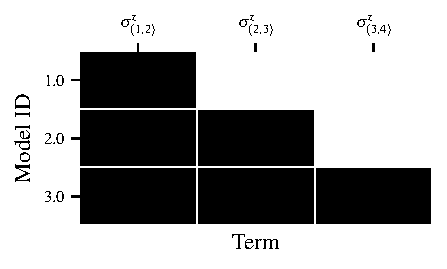
\includegraphics[width=0.45\textwidth]{qmla_run_data/Jan_17//21_53/instances/qmla_1/composition_of_models.pdf}
            \label{fig:qmla_model_composition}
        }
        \qquad
        \subfloat[]{
            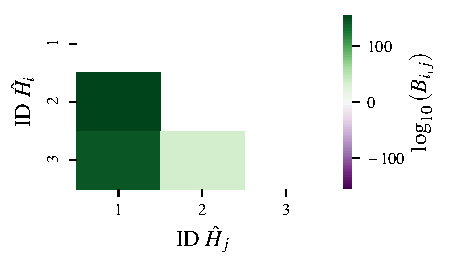
\includegraphics[width=0.45\textwidth]{qmla_run_data/Jan_17//21_53/instances/qmla_1/bayes_factors.pdf}
            \label{fig:qmla_bayes_factors}
        }
        \qquad
        \subfloat[]{
            \includegraphics[width=0.45\textwidth]{qmla_run_data/Jan_17//21_53/instances/qmla_1/comparisons/BF_1_2.pdf}
            \label{fig:qmla_bayes_factor_comparison}
        }
        \qquad
        \subfloat[]{
            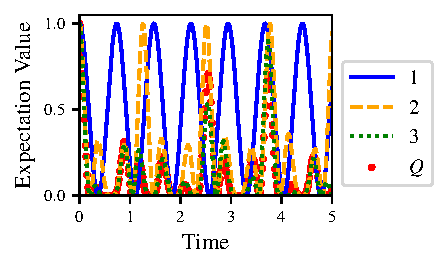
\includegraphics[width=0.45\textwidth]{qmla_run_data/Jan_17//21_53/instances/qmla_1/branches/dynamics_branch_1.pdf}
            \label{fig:qmla_branch_dynamics}
        }
        \qquad
        \subfloat[]{
            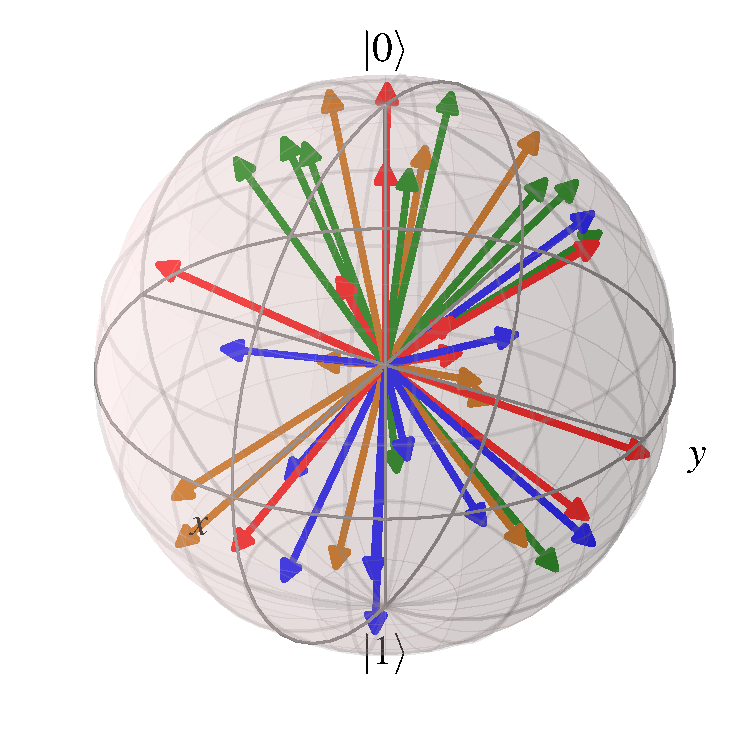
\includegraphics[width=0.25\textwidth]{qmla_run_data/Jan_17//21_53/instances/qmla_1/probes_bloch_sphere.pdf}
            \label{fig:qmla_training_probes}
        }
    \end{center}
    \caption[Instance plots]{
        \gls{qmla} plots; found within instance directory e.g. \ttt{Jan\_01/01\_23/instances/qmla\_1}. 
        \textbf{(a)} \ttt{composition\_of\_models}: constituent terms of all considered models, indexed by their model IDs.
        \textbf{(b)} \ttt{bayes\_factors}: \glsentrylong{bf} comparisons between all models. 
        \gls{bf} are read as $B_{a,b}$ where $a$ is the model with lower ID, 
            e.g. $B_{1,2}$ rather than $B_{2,1}$. Thus $B > 0 (<0)$ indicates $a$ ($b$) is the stronger model.
        \textbf{(c)} \ttt{comparisons/BF\_1\_2}: direct comparison between models with IDs 1 and 2, 
            showing their reproduction of the system dynamics, 
            as well as the times (experiments) against which the \gls{bf} was calculated. 
        \textbf{(d)} \ttt{branches/dynamics\_branch\_1}: dynamics of all models considered on the branch. 
        \textbf{(e)} \ttt{probes\_bloch\_sphere}: probes used for training models in this instance (only showing 1-qubit versions).
    }
    \label{fig:instance_plots}
\end{figure}

\subsection{\Gls{run} analysis}
Considering a number of \glspl{instance} together is a \gls{run}. 
In general, this is the level of analysis of most interest: 
    an individual instance is liable to errors due to the probabilistic nature of 
    the model training and generation subroutines. 
On average, however, we expect those elements to perform well, 
    so across a significant number of instances, we expect the average outcomes to be meaningful. 
\par 

Each results directory has an \ttt{analyse.sh} script to generate plots at the \gls{run} level. 
\begin{lstlisting}[
    label=listing:analysing_run,
    caption={Analysing QMLA run.},
    language=Bash
]
cd results/Jan_01/01_23
./analyse.sh
\end{lstlisting}

Run level analysis are held in the main results directory and several sub-directories created by the \ttt{analyse} script. 
Here, we recommend running a number of instances with very few resources so that the test finishes quickly\footnote{This run will take about ten minutes}. 
The results will therefore be meaningless, but allow fo elucidation of the resultant plots. 
First, reconfigure some settings of \cref{listing:local_launch} and launch again.
\begin{lstlisting}[
    label=listing:example_es_qhl_run,
    caption={\ttt{local\_launch} configuration for QMLA.},
    language=Bash
]
num_instances=10
exp=20
prt=100
run_qhl=0
exploration_strategy=ExampleBasic
\end{lstlisting}
\par 

Some of the generated analysis are shown in \crefrange{fig:run_plots}{fig:run_dynamics}. 
The number of instances for each model, i.e. their \emph{\glspl{win rate}} are given in \cref{fig:qmla_win_rates}.
Quantitative comparisons between candidate models, i.e. \glspl{bf} are in \cref{fig:qmla_bayes_factors}.
Irrespecitve of the champion models, the rate with which each term is found in the champion model ($\hat{t} \in \hp$)
    indicates the likelihood that the term is really present;
    these rates -- along with the parameter values learned -- are shown in \cref{fig:qmla_branch_dynamics}.
The champion model from each instance can attempt to reproduce system dynamics: 
    we group together these reproductions for each model in \cref{fig:run_dynamics}. 

\begin{figure}[H]
    \begin{center}
        \subfloat[]{
            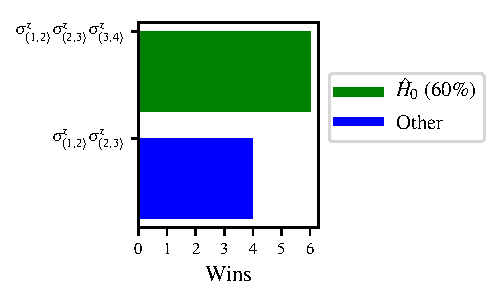
\includegraphics{qmla_run_data/Jan_17/22_27/performance/model_wins.pdf}
            \label{fig:qmla_win_rates}
        }
        \qquad
        \subfloat[]{
            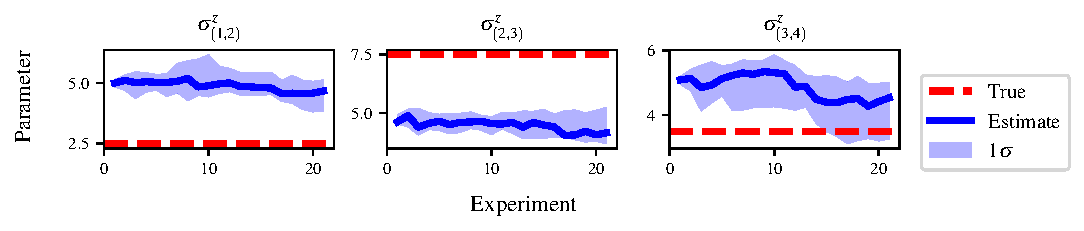
\includegraphics{qmla_run_data/Jan_17/22_27/champion_models/params_pauliSet_1J2_zJz_d4+pauliSet_2J3_zJz_d4+pauliSet_3J4_zJz_d4.pdf}
            \label{fig:qmla_bayes_factors}
        }
        \qquad
        \subfloat[]{
            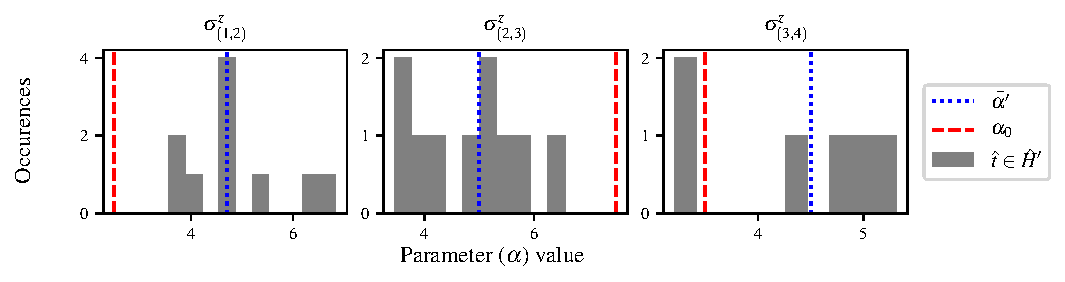
\includegraphics{qmla_run_data/Jan_17/22_27/champion_models/terms_and_params.pdf}
            \label{fig:qmla_branch_dynamics}
        }
    \end{center}
    \caption[Run plots]{
        \gls{qmla} run plots; found within run directory e.g. \ttt{Jan\_01/01\_23/}. 
        \textbf{(a)} \ttt{performace/model\_wins}: number of instance wins achieved by each model. 
        \textbf{(b)} \ttt{champion\_models/params\_params\_pauliSet\_1J2\_zJz\_d4+pauliSet\_2J3\_zJz\_d4+pauliSet\_3J4\_zJz\_d4}: 
            parameter estimation progression for the true model, only for the instances where it was deemed champion. 
        \textbf{(c)} \ttt{champion\_models/terms\_and\_params}: 
            histogram of parameter values found for each term which appears in any champion model,
            with the true parameter ($\alpha_0$) in red and the median learned parameter ($\alpha^{\prime}$) in blue.
    }
    \label{fig:run_plots}
\end{figure}

\begin{figure}[H]
    \begin{center}
        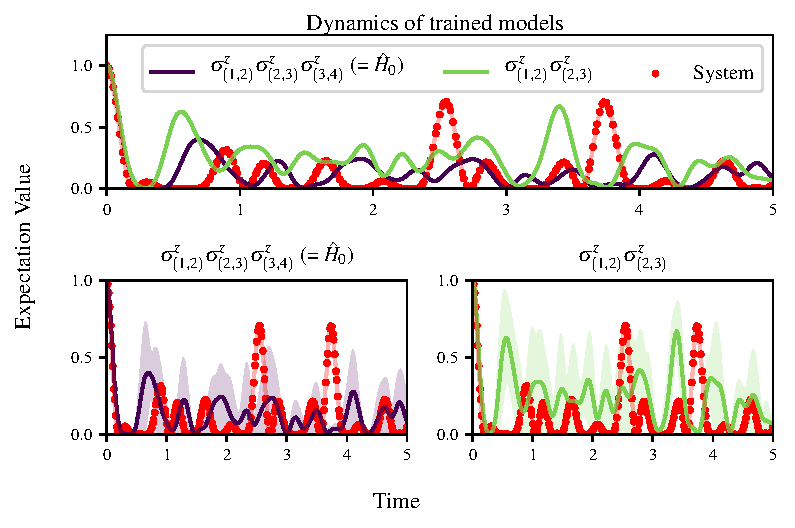
\includegraphics{qmla_run_data/Jan_17/22_27/performance/dynamics.pdf}
    \end{center}
    \caption{
        Run plot \ttt{performace/dynamics}: median dynamics of the champion models. 
        The models which won most instances are shown together in the top panel, 
        and individually in the lower panels. 
        The median dynamics from the models' learnings in its winning instances are shown, 
        with the shaded region indicating the 66\% confidence region. 
    }
    \label{fig:run_dynamics}
\end{figure}



\section{Parallel implementation}


% TODO use backslash package

